% Source : http://tex.stackexchange.com/questions/31336/how-can-i-display-an-array-as-in-the-data-structure-from-computer-science-not-t

\documentclass{article}
	\usepackage{tikz}
	\usetikzlibrary{calc}


\begin{document}

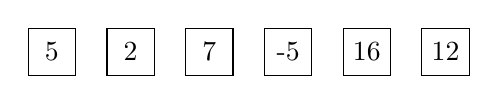
\begin{tikzpicture}
	\coordinate (s) at (0,0);
	\foreach \num in {5,2,7,-5,16,12}{
		\node[minimum size=6mm, draw, rectangle] at (s) {\num};
		\coordinate (s) at ($(s) + (1,0)$);
	}
\end{tikzpicture}

\end{document}
